%from ChaosBook.org \Chapter{flows}{27aug2008}{Go with the flow}
% $Author$ $Date$

In this chapter we present a simple example of symmetry reduction applied to
Lorenz flow.

%%%%%%%%%%%%%%%%%%%%%%%%%%%%%%%%%%%%%%%%%%%%%%%%%%%%%
\SFIG{lorenz_less_ugly_bm}{}
{Lorenz ``butterfly'' strange attractor.  (J. Halcrow)}
{LorenzAttrct}
%%%%%%%%%%%%%%%%%%%%%%%%%%%%%%%%%%%%%%%%%%%%%%%%%%%%%

%%%%%%%%%%%%%%%%%%%%%%%%%%%%%%%%%%%%%%%%%%%%%%%%%%%%%%%%%%%%%%%%%%%%%%%%%%
\section{Lorenz strange attractor\label{exmp:Lorenz}}
% Predrag                           17feb2008
% Predrag                           10dec2007
% Predrag                           20sep2007
% transferred from halcrow/blog/TEX/lorenz.tex
Edward Lorenz arrived at the equation \refeq{eq:lorenz}
\index{Lorenz flow}\index{Rayleigh-Benard flow}
\beq
\dot{\ssp}=\pVeloc(\ssp)
    =
    \left[
        \begin{array}{c}
\dot{x} \\ \dot{y} \\ \dot{z}
    \end{array}
    \right]
    =
    \left[
        \begin{array}{c}
\sigma (y-x) \\
\rho x - y -xz \\
xy -bz
    \end{array}
    \right]
\ee{Lorenz}
by a drastic simplification of
the Rayleigh-Benard flow. %\rf{lorenz63}.
Lorenz fixed
$\sigma = 10$, $ b= 8/3$,
and varied the ``Rayleigh number'' $\rho$. For
$0 < \rho < 1$ the \eqv\ $\EQV{0} =(0,0,0)$
at the origin is attractive.
At $ \rho = 1$  it undergoes a pitchfork
bifurcation into a pair of \eqva\ at
\index{equilibrium!Lorenz flow}
\beq
\ssp_{\EQV{1,2}} = (\pm \sqrt{b(\rho-1)}, \pm \sqrt{b(\rho-1)}, \rho-1)
\,,
\ee{LorEqva}
We shall not explore the Lorenz flow dependence on the $\rho$
parameter in what follows, but here is a brief synopsis: the
$\EQV{0}$  $1$\dmn\ unstable manifold closes into a
homoclinic orbit at $\rho=13.56\dots$. Beyond that, an infinity
of associated \po s are generated, until $\rho = 24.74\dots$,
where $\EQV{1,2}$ undergo a Hopf bifurcation.
    \PC{ \reffig{LorenzAttrct} .eps still too big}

All computations that follow
will be performed for the Lorenz parameter choice
\(
    \sigma = 10, b= 8/3, \rho = 28
\,.
\)
For these parameter values the long-time dynamics is confined to
the strange attractor
depicted in  \reffig{LorenzAttrct}.

\section{Sections of Lorenz flow}\label{exmp:LorenzSect}
% from ChaosBook.org \Chapter{maps}{13jun2008}{Discrete time dynamics}
% predrag  2009-02-22
% Predrag                           04apr2008
% Predrag                           19jan2008
% moved to here from halcrow/blog/TEX/lorenz.tex

%%%%%%%%%%%%%%%%%%%%%%%%%%%%%%%%%%%%%%%%%%%%%%%%%%%%%
\FIG{{
(a)~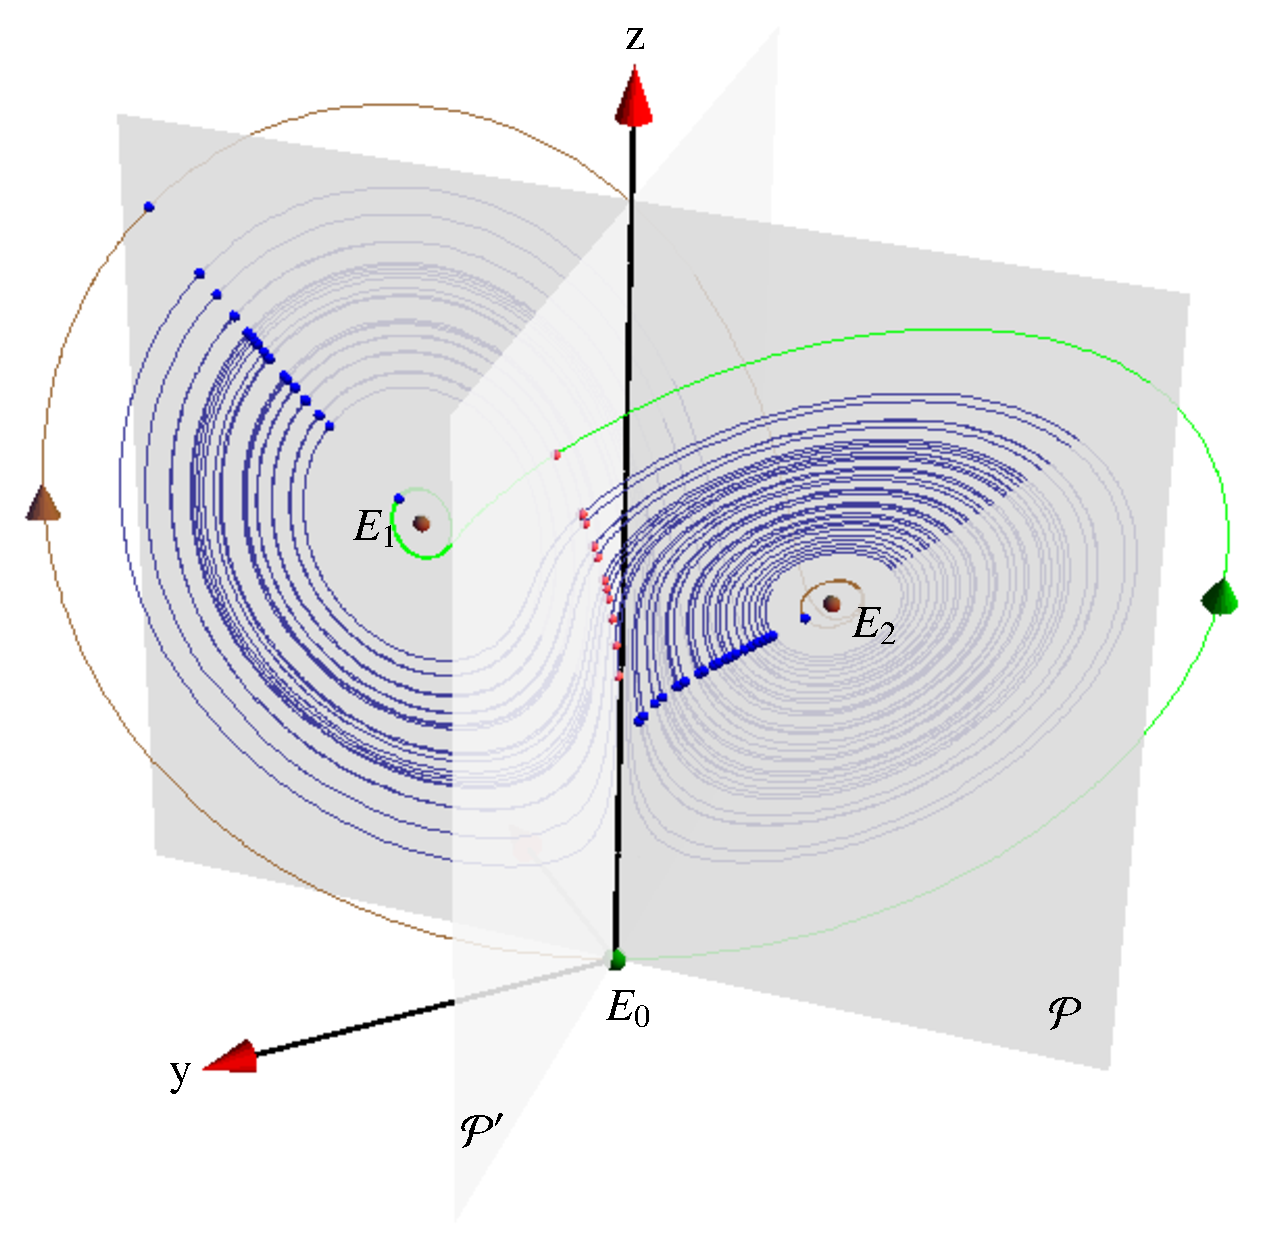
\includegraphics[width=0.48\textwidth]{../figs/lorenz2Poinc}
(b)~\raisebox{1.0ex}{
    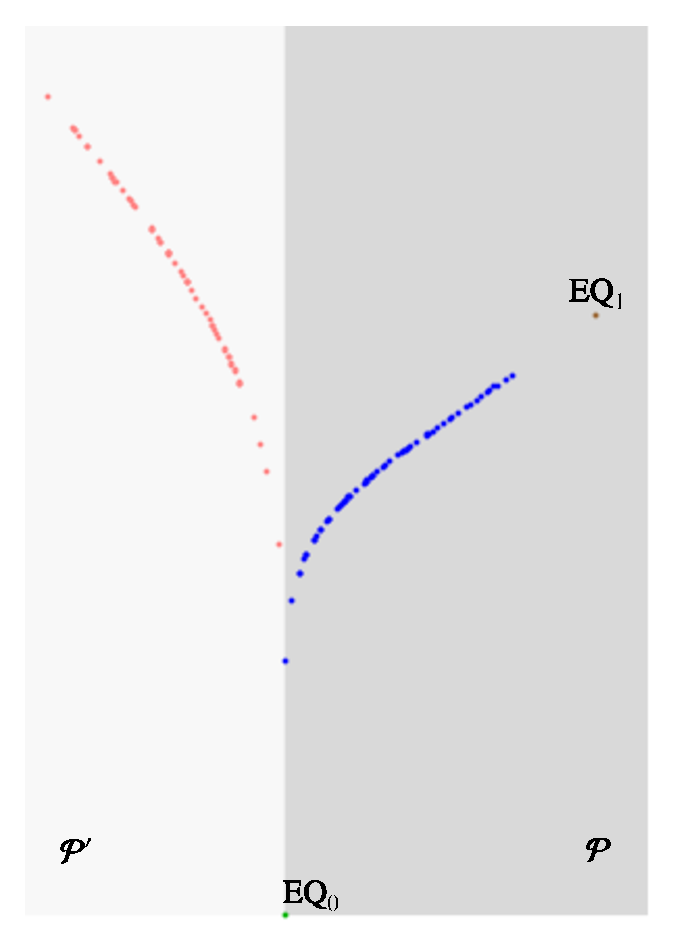
\includegraphics[width=0.30\textwidth]{../figs/lorenz2Poinc2D}
                    }}
}{}{
(a) Lorenz flow \reffig{LorenzAttrct}
cut by  $y=x$ Poincar\'e section plane $\PoincS$
through the $z$ axis and both $\EQV{1,2}$ \eqva.
Points where flow pierces into section % $\PoincS$
are marked by dots.
To aid visualization of the flow near the $\EQV{0}$ \eqv,
the flow is cut by the second Poincar\'e section,  $\PoincS'$,
through $y=-x$ and the $z$ axis.
% Marking the ingoing sections yields a symmetric image.
(b) Poincar\'e sections $\PoincS$ and $\PoincS'$ laid side-by-side.
The singular nature of these sections close to $\EQV{0}$ will be
elucidated in \refsect{exmp:LorenzStab}
and \reffig{fig:PoincLorenz}\,(b).
%       \(\sigma = 10, b= 8/3, \rho = 28\,.\)
}{fig:LorenzSect}
%%%%%%%%%%%%%%%%%%%%%%%%%%%%%%%%%%%%%%%%%%%%%%%%%%%%%


The plane $\PoincS$
fixed by the $x=y$ diagonal and
the $z$-axis depicted in \reffig{fig:LorenzSect} is
a natural choice of a Poincar\'e section of the Lorenz
flow of \reffig{LorenzAttrct},
as it contains all three  \eqva, $\ssp_{\EQV{0}} =(0,0,0)$
and the \refeq{LorEqva} pair $\EQV{1,2}$.
A section has
to be supplemented with an orientation
condition: here
points where flow pierces \emph{into} the section
are marked by dots.
    \index{Lorenz flow}\index{equilibrium!Lorenz flow}
    %
    \PC{\reffig{fig:LorenzSect}\,(b): generate
        .eps from lorenz2Poinc2D.pdf,
        this is the old version. Raise it a bit.
        }

$\EQV{1,2}$ are centers of out-spirals, and close to them  the
section is transverse to the flow. However, close to  $\EQV{0}$
trajectories pass the $z$-axis either by crossing the section
$\PoincS$ or staying on the viewer's side. We are free to
deploy as many sections as we wish: in order to capture the
whole flow in this neighborhood we add the second Poincar\'e
section, $\PoincS'$, through the $y=-x$ diagonal and the
$z$-axis. Together the two sections,
\reffig{fig:LorenzSect}\,(b), capture the whole flow near
$\EQV{0}$. The dynamics on the sections appear very singular.
We explain this singularity in \refsect{exmp:LorenzStab}, and
postpone construction of a Poincar\'e return map to
\refsect{exmp:LorenzD1}.

\subsection{Stability of Lorenz flow \eqva}\label{exmp:LorenzStab}
%from ChaosBook.org \Chapter{stability}{21feb2009}{Local stability}
% Predrag: 2009-02-22
For the  Lorenz
\refeq{Lorenz} flow the {\stabmat} is
  \beq
{\Mvar_{Lor}} =
  \left(\barr{ccc}
    -\sigma  & \sigma &  0 \\
    \rho-z   &   -1   &  x \\
       y     &    x   & -b
    \earr\right)
  \,.
  \ee{LorLinrz}

%%%%%%%%%%%%%%%%%%%%%%%%%%%%%%%%%%%%%%%%%%%%%%%%%%%%%%%%%%%%%%%%%%%%%%%%%%
% Predrag                           04apr2008
% Predrag                           19jan2008
% moved to here from halcrow/blog/TEX/lorenz.tex
%
% \example{Stability of Lorenz flow \eqva:}{ \label{exmp:LorenzStab}
\index{Lorenz flow}
A glance at \reffig{fig:LorenzSect} suggests that the
flow is organized by its 3 \eqva, so lets have a closer look at
their stable/unstable manifolds.

The $\EQV{0}$ \eqv\  {\stabmat} \refeq{LorLinrz}
evaluated at $\ssp_{\EQV{0}} =(0,0,0)$ is block-diagonal.
The $z$-axis is an eigen\-vector
with a contracting eigenvalue $\eigExp[2]=-b$.
From \refeq{trA-Lorenz} it follows that all $[x,y]$ areas
shrink at rate $-(\sigma +1)$. Indeed, the
$[x,y]$ submatrix
\beq
{\Mvar^{-}} =
  \left(\barr{cc}
    -\sigma  & \sigma  \\
    \rho     &   -1
    \earr\right)
\ee{LorzEQ0plus}
has a real expanding/contracting eigenvalue pair
$\eigExp[1,3]=
-(\sigma +1)/2 \pm \sqrt{(\sigma-1)^2/4 + \rho \sigma}$,
with the right eigen\-vectors $\jEigvec[1]$,  $\jEigvec[3]$
in the $[x,y]$ plane, given by (either) column of
the projection operator
\beq
{\PP_i} = \frac{\Mvar^{-} -\eigExp[j] \matId}{\eigExp[{i}]-\eigExp[{j}]}
 = \frac{1}{\eigExp[{i}]-\eigExp[{j}]}
  \left(\barr{cc}
    -\sigma  - \eigExp[{j}] & \sigma  \\
                 \rho   &   -1-\eigExp[{j}]
    \earr\right)
  \,,\qquad i \neq j \in \{1,3\}
  \,.
\ee{LorzEQ0eVect}


$\EQV{1,2}$ \eqva\ have no symmetry, so
their eigenvalues are given by
the roots of a cubic equation, the secular determinant
$\det(\Mvar - \Lyap  \matId)=0$:
\beq
% \EQV{0}~~ &:& \;\; (\eigExp[+],\Lyap_-,\Lyap_s)
%    =  (-(\sigma +1)/2 \pm \sqrt{(\sigma-1)^2/4 + \rho \sigma}, -b)
% \EQV{1,2} &:&  \;\;   \mbox{}
     \Lyap^3+\Lyap^2(\sigma+b+1)+\Lyap b(\sigma+\rho)+2\sigma b (\rho-1) = 0
\,.
\label{LorenzEqQigs}
\eeq
For $\rho > 24.74$, $\EQV{1,2}$ have one stable real eigenvalue and
one unstable complex conjugate pair, % as solutions to \refeq{LorenzEqQigs},
leading to a spiral-out instability and the strange attractor
depicted in  \reffig{LorenzAttrct}.


%%%%%%%%%%%%%%%%%%%%%%%%%%%%%%%%%%%%%%%%%%%%%%%%%%%%%
\FIG{
(a)  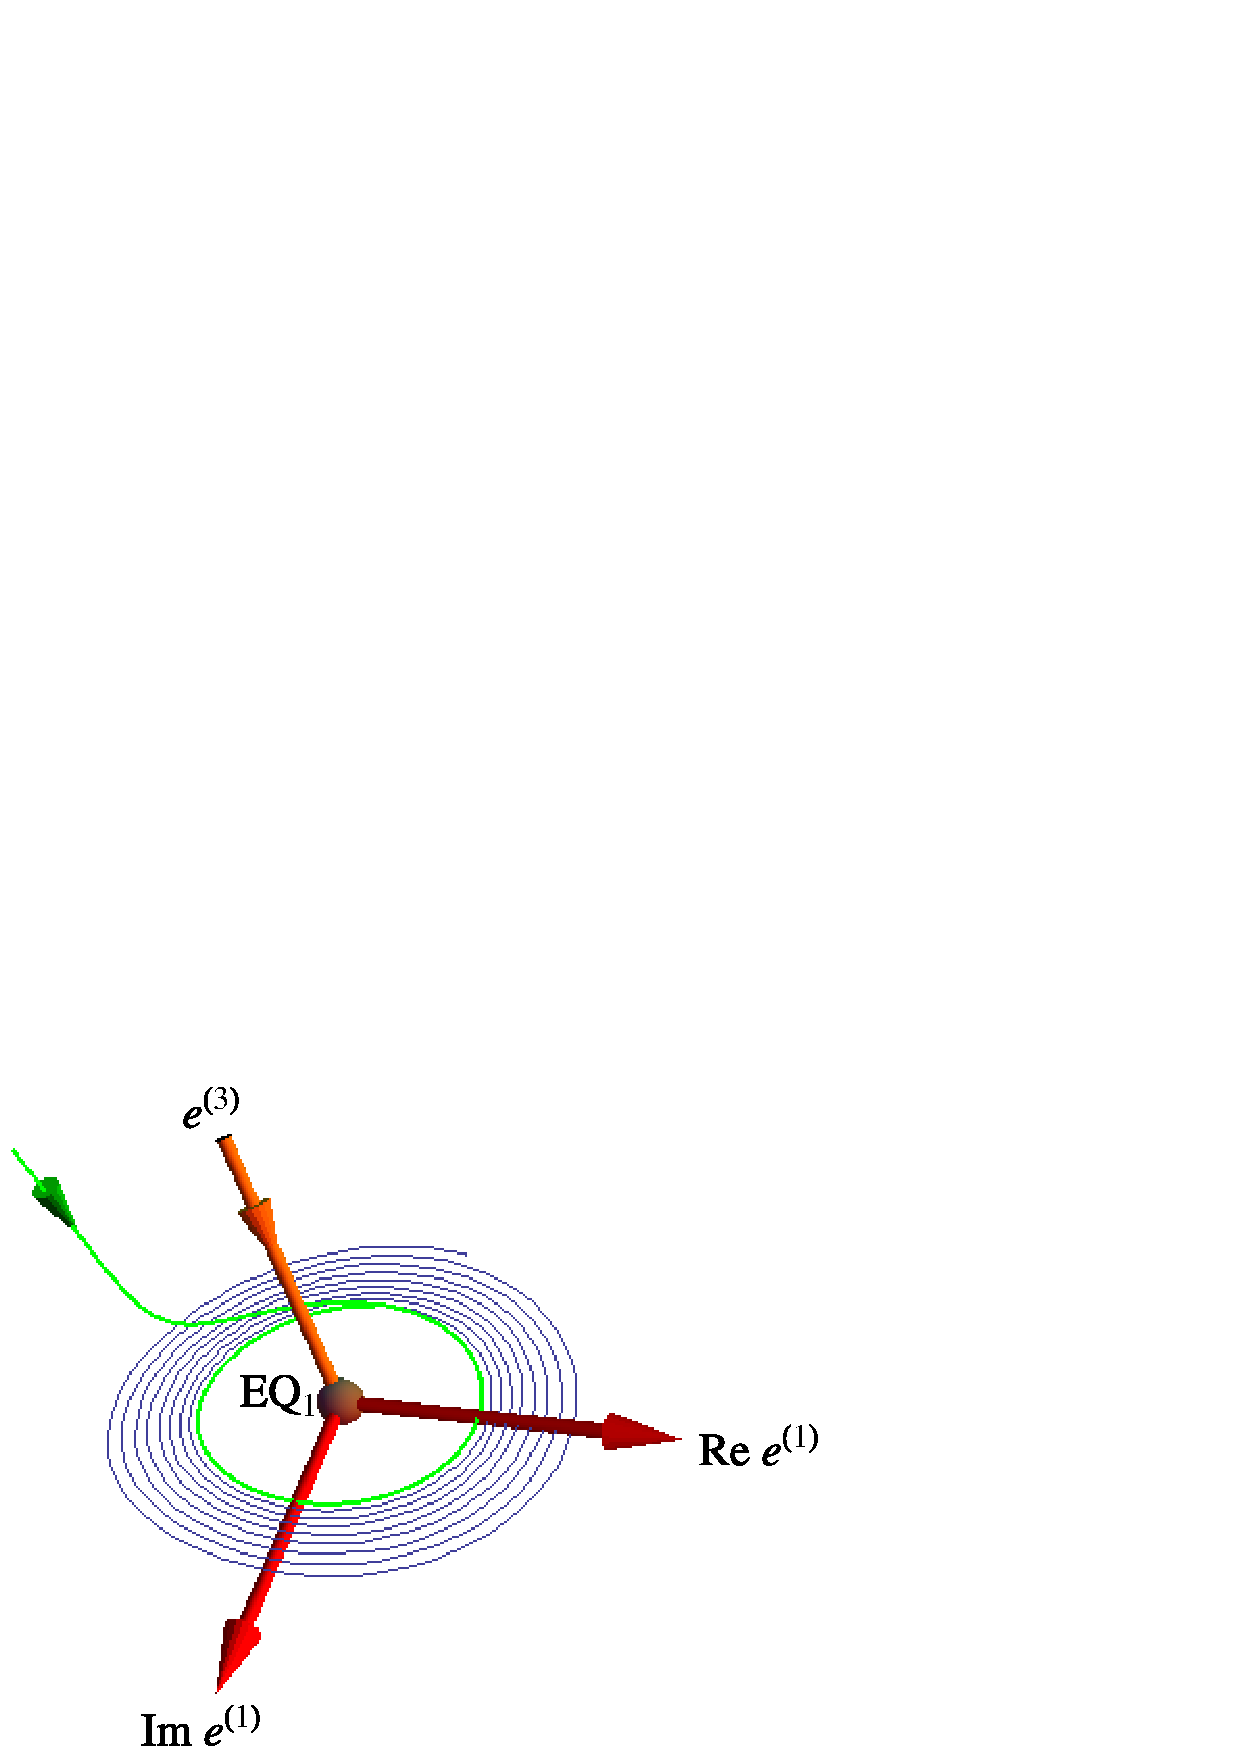
\includegraphics[width=0.36\textwidth]{../figs/lorenzPolarManifDetail1}  %.png}
(b)  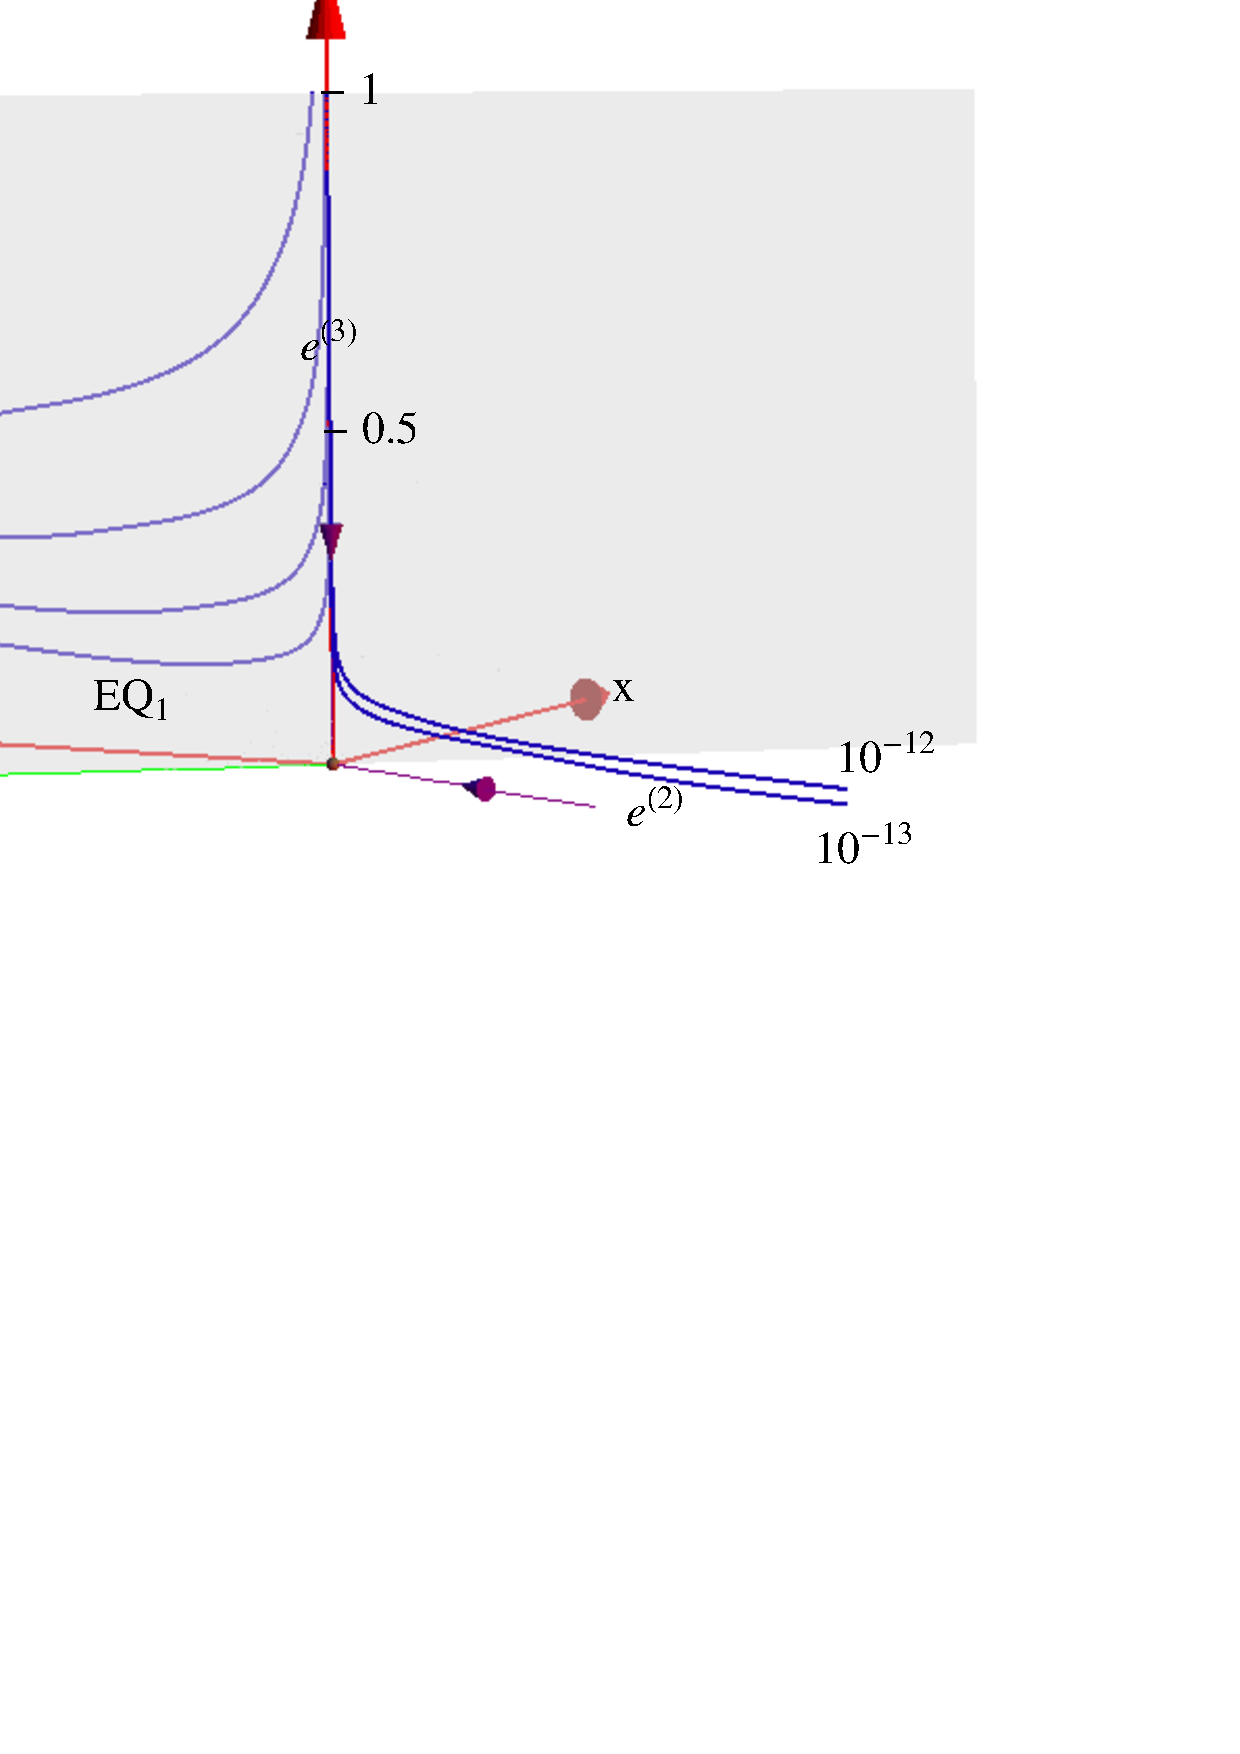
\includegraphics[width=0.56\textwidth]{../figs/lorenzSaddle0}  %.png}
}{}{
(a) A perspective view of the linearized Lorenz flow near $\EQV{1}$ \eqv,
see \reffig{fig:LorenzSect}\,(a).
The unstable eigenplane of $\EQV{1}$ is
spanned by \Re\jEigvec[1]\ and \Im\jEigvec[1]. The
stable eigen\-vector  $\jEigvec[3]$.
(b) Lorenz flow near the $\EQV{0}$ \eqv: unstable
eigen\-vector  $\jEigvec[1]$,
stable eigen\-vectors  $\jEigvec[2]$,  $\jEigvec[3]$.
Trajectories initiated at distances
$10^{-8}$ $\cdots$ $10^{-12}$, $10^{-13}$ away from the
$z$-axis exit finite distance from $\EQV{0}$  along the
$(\jEigvec[1],\jEigvec[2])$ eigen\-vectors plane.
%starting at approximate from the heteroclinic connection from
%$\EQV{1}$ to $\EQV{0}$.
Due to the strong $\eigExp[1]$ expansion, the
$\EQV{0}$ \eqv\ is, for all practical purposes,
unreachable, and the  $\EQV{1} \to \EQV{0}$ heteroclinic connection
never observed in simulations such as
\reffig{LorenzAttrct}.
%(E. Siminos; continued in \reffig{fig:PoincLorenz}.)
    }{fig:LorenzEQ1} %fig:LorenzEQ0}
%%%%%%%%%%%%%%%%%%%%%%%%%%%%%%%%%%%%%%%%%%%%%%%%%%%%%

As all numerical plots of the Lorenz flow are
here carried out for the Lorenz parameter choice
\(
    \sigma = 10, b= 8/3, \rho = 28
\,,
\)
we note the values of these eigenvalues for future reference,
\beq
\barr{lcrl}
\EQV{0}:~
(\eigExp[1],\eigExp[2], \eigExp[3])
    &=& (\,11.83\,,~-2.666,& -22.83\,)   \\
\EQV{1}:~
(\eigRe[1] \pm\,i\,\eigIm[1],\eigExp[3])
    &=& (\,\,0.094\,\pm i\,10.19,\,& -13.85\,) \,, \\
\earr
\label{EqLorenzStab}
\eeq
as
well as the rotation period
$T_{\EQV{1}} = 2\pi/\eigIm[1]$ about $\EQV{1}$,
and the  associated expansion/contraction multipliers
$\ExpaEig^{(i)} = \exp(\eigRe[j] T_{\EQV{1}})$
per a spiral-out turn:
\index{turnover time}
\index{time!turnover}
\beq
T_{\EQV{1}} =  0.6163 \,, \qquad
(\ExpaEig^{(1)},\ExpaEig^{(3)})
   = (\,1.060 \,, 1.957\times 10^{-4} \,)
\,.
\label{EqLorenzMltp}
\eeq
We learn that the typical turnover time scale in this problem is
of order $T \approx T_{\EQV{1}} \approx 1$
(and not, let us say, 1000, or $10^{-2}$). Combined with
the contraction rate \refeq{trA-Lorenz}, this tells us that
the Lorenz flow strongly contracts \statesp\ volumes, by factor of
$ \approx 10^{-4}$ per mean turnover time.

In the $\EQV{1}$ neighborhood the unstable manifold
trajectories slowly spiral out, with
very small radial  per-turn expansion multiplier
$\ExpaEig^{(1)} \simeq  1.06$,
and very strong contraction multiplier
$\ExpaEig^{(3)}  \simeq 10^{-4}$
onto the unstable manifold,
\reffig{fig:LorenzEQ1}\,(a).
This contraction confines, for all practical purposes,
the Lorenz attractor to a 2\dmn\ surface
evident in the section \reffig{fig:LorenzSect}.

%The unstable eigenplane is defined by eigen\-vectors
%$ \Re\jEigvec[2]=(-0.4955, -0.2010, -0.8450)
%  \Im\jEigvec[2]=(0.5325, -0.8464, 0) $
%along the stable eigen\-vector of $\EQV{1}$, $(0.8557, -0.3298, -0.3988) $.

In the $\ssp_{\EQV{0}} = (0,0,0)$ \eqv\ neighborhood the extremely strong
$\eigExp[3] \simeq -23$ contraction along the $\jEigvec[3]$ direction
confines the hyperbolic dynamics near $\EQV{0}$ to the plane
spanned by the unstable eigen\-vector $\jEigvec[1]$,
with $\eigExp[1] \simeq 12$, and
the slowest contraction rate eigen\-vector $\jEigvec[2]$
along the $z$-axis, with $\eigExp[2] \simeq - 3$.
In this plane the strong expansion % $\eigExp[1] \simeq 18$ % JFG: 12?
along $\jEigvec[1]$ overwhelms the
slow  $\eigExp[2] \simeq - 3$ contraction down the $z$-axis,
making it extremely unlikely for a random trajectory
to approach $\EQV{0}$, \reffig{fig:LorenzEQ1}\,(b).
Thus linearization suffices to describe analytically the singular
dip in the Poincar\'e sections of
\reffig{fig:LorenzSect}, and the empirical scarcity
of trajectories close to $\EQV{0}$.

%%%%%%%%%%%%%%%%%%%%%%%%%%%%%%%%%%%%%%%%%%%%%%%%%%%%%%%%%%%%%%%%%%%%%%%%%%
\section{Lorenz flow: Global portrait}\label{exmp:LorenzGlob}
% Predrag                           04apr2008
% Predrag                           19jan2008
% moved to here from halcrow/blog/TEX/lorenz.tex
\index{Lorenz flow}

As the $\EQV{1}$ unstable manifold spirals out,
the strip that starts out in the section above $\EQV{1}$
in \reffig{fig:LorenzSect} cuts across the
$z$-axis invariant subspace. This strip necessarily contains a
heteroclinic orbit that hits the $z$-axis
head on, and in infinite time (but exponentially
fast) descends all the way to $\EQV{0}$.
\PC{This needs more explaining. As
    $\EQV{0}$ has 2 contracting dimensions (and fluids will
    have 50,000), whole volumes get scrunched into $\EQV{0}$,
    not just 1\dmn\ heteroclinic orbits.
   }


How? As in the neighborhood of the
$\EQV{0}$ \eqv\ the dynamics is linear
(see \reffig{fig:LorenzEQ1}\,(a)), there
is no need to integrate numerically the final segment
of the heteroclinic
connection - it is sufficient to bring a trajectory
a small distance away from $\EQV{0}$, continue
analytically to a small distance
beyond $\EQV{0}$,
then resume the numerical integration.

What happens next? Trajectories to the left of $z$-axis shoot
off along the $\jEigvec[1]$ direction, and those to the
right along $-\jEigvec[1]$. As along the $\jEigvec[1]$ direction
$xy >0$, the nonlinear term in the $\dot{z}$ equation \refeq{Lorenz}
bends both branches of the
$\EQV{0}$ unstable manifold $W^u(\EQV{0})$ upwards.
Then $\ldots$ - never mind.
Best to postpone the completion of this narrative to
\refsect{exmp:LorenzD1}, where the discrete
symmetry of Lorenz flow will help us streamline the analysis.
As we shall show, what we already know about the 3 \eqva\ and
their stable/unstable manifolds suffices to completely pin down
the topology of Lorenz flow.


\subsection{Lorenz flow \statesp\ contraction}\label{exmp:LorenzContr}
\index{Lorenz flow}

The Lorenz flow is volume contracting,
\beq
\pde_i \pVeloc_i
 = \sum_{i=1}^{3} \eigExp[i](\ssp,t)
= -\sigma -b -1
    \,,
\ee{trA-Lorenz}
at a constant, coordinate- and $\rho$-independent rate, set by
Lorenz to $\pde_i \pVeloc_i = -13.66$ . As for \po s and for
long time averages there is no contraction/expansion along the
flow, $\eigExp[\parallel]=0$, and the sum of $\eigExp[i]$ is
constant by \refeq{trA-Lorenz}, there is only one independent
exponent $\eigExp[i]$ to compute.


\section{Desymmetrization of the Lorenz flow}\label{exmp:LorenzD1}
%from ChaosBook.org \Chapter{discrete}{5sep2008}{World in a mirror}

The vector field in Lorenz equations  \refeq{Lorenz} is
equivariant under the action of  cyclic group
$\Ztwo = \{e,\Rot{1/2}\}$
acting on \Rls{3}\ by a $\pi$ rotation about the $z$ axis,
\[
    \Rot{1/2}(x,y,z) = (-x,-y,z)\,.
\]
%This transformation can be considered as either as rotation by
%$\pi$ around the $z$ axis (hence the group \Ztwo) or as a
%reflection about the origin in a plane perpendicular to the
%$z$-axis (hence the group \Dn{1}.)
\index{Lorenz flow!symmetry}
%         } %end \example{Discrete symmetries of $3d$ flow

%%%%%%%%%%%%%%%%%%%%%%%%%%%%%%%%%%%%%%%%%%%%%%%%%%%%%%%%%%%%%%%%%%%%%%%%%%
% \example{Desymmetrization of Lorenz flow:}{ \label{exmp:LorenzD1}
% Predrag                           04apr2008
% Predrag                           19jan2008
% moved to here from halcrow/blog/TEX/lorenz.tex
\index{Lorenz flow}
Lorenz equation \refeq{Lorenz} is invariant under
the action of order-2 group $\Ztwo = \{e,\Rot{1/2}\}$, where
 $\Rot{1/2}$ is $[x,y]$-plane, constant $z$  rotation by $\pi$ about the $z$-axis:
\beq
(x,y,z) \to \Rot{1/2}(x,y,z) = (-x,-y,z) \,.
\ee{LorenzR}
$(\Rot{1/2})^2=1$ condition decomposes the \statesp\ into two
linearly irreducible subspaces
$\pS = \pS^+ \oplus \pS^-$,
the $z$-axis $\pS^+$ and
the $[x,y]$ plane $\pS^-$, with
projection operators onto the two subspaces given by
 \beq
 \PP^+ = \frac{1}{2}(1 + \Rot{1/2})
 =   \left(\barr{ccc}
    0  &  0 & 0  \\
    0  &  0 & 0 \\
    0  &  0 & 1
    \earr\right)
     ,\quad
 \PP^- = \frac{1}{2}(1 - \Rot{1/2})
  =   \left(\barr{ccc}
    1  &  0 & 0  \\
    0  &  1 & 0 \\
    0  &  0 & 0
    \earr\right)
\,.
 \label{projOp:sig}
 \eeq
As the flow is $\Ztwo$-invariant, so is its linearization
$\dot{\ssp} = \Mvar \ssp$. Evaluated at $\EQV{0}$, $\Mvar$
commutes with  $\Rot{1/2}$, and,
as we have already seen in  \refsect{exmp:LorenzStab},
the $\EQV{0}$ {\stabmat}
decomposes into $[x,y]$ and $z$ blocks.

The 1\dmn\ $\pS^+$ subspace is
the fixed-point subspace of $\Ztwo$, with the $z$-axis
points left \emph{point-wise} invariant under the group
action
\beq
\mbox{Fix}(\Ztwo) =
   \{ \ssp \in \pS^+ : \mathbf{g} \, \ssp = \ssp \mbox{ for } g \in \{e,\Rot{1/2}\} \}
\,.
\ee{dscr:LorFPsubsp}
However, a point $\ssp(t)$ in $\mbox{Fix}(G)$ moves with time,
but remains within $\ssp(t) \subseteq \mbox{Fix}(G)$ for all
times; the  subspace $\pS^+ = \mbox{Fix}(G)$ is {\em flow
invariant}. In case at hand this jargon is a bit of an
overkill: clearly for $(x,y)=(0,0)$ the full \statesp\ Lorenz
equation \refeq{Lorenz} is reduced to the exponential
contraction to the $\EQV{0}$ \eqv,
\beq
\dot{z} = -b \, z
\,.
\ee{LorenzZaxis}
% which is the reason why you never see this decomposition discussed
% in literature. Even though
However, for flows in higher-dimensional \statesp s the
flow-invariant $\pS^+$ subspace can itself be high-dimensional, with
interesting dynamics of its own.
Even in this simple case this subspace plays an important role
as a topological obstruction, with
the number of winds of a trajectory around it providing
a natural symbolic dynamics.

The $\pS^-$ subspace is, however, {\em not} flow-invariant, as the nonlinear
terms $\dot{z}=xy - bz$ in the Lorenz equation \refeq{Lorenz}
send all initial conditions within
$\pS^-=(x(0),y(0),0)$ into the full, $z(t) \neq 0$ \statesp\  $\pS$.
The $\Rot{1/2}$ symmetry is nevertheless very useful.

By taking as a Poincar\'e section % $\PoincS$
any  $\Rot{1/2}$-invariant, infinite-extent, non-self-inter\-sect\-ing
surface that contains the
$z$ axis, the \statesp\ is divided into a half-space fundamental
domain $\tilde{\pS}=\pS/\Ztwo$ and its $180^o$ rotation $\Rot{1/2}\tilde{\pS}$.
An example is afforded by the $\PoincS$ plane section of
the Lorenz flow in \reffig{fig:LorenzSect}. Take
the  fundamental domain $\tilde{\pS}$ to be the half-space between the
viewer and $\PoincS$. Then the full Lorenz
flow is captured by re-injecting back into $\tilde{\pS}$
any trajectory that exits it, by a rotation of $\pi$ around the $z$ axis.

%%%%%%%%%%%%%%%%%%%%%%%%%%%%%%%%%%%%%%%%%%%%%%%%%%%%%%%%%%%%%%%%%%
\FIG{
(a)~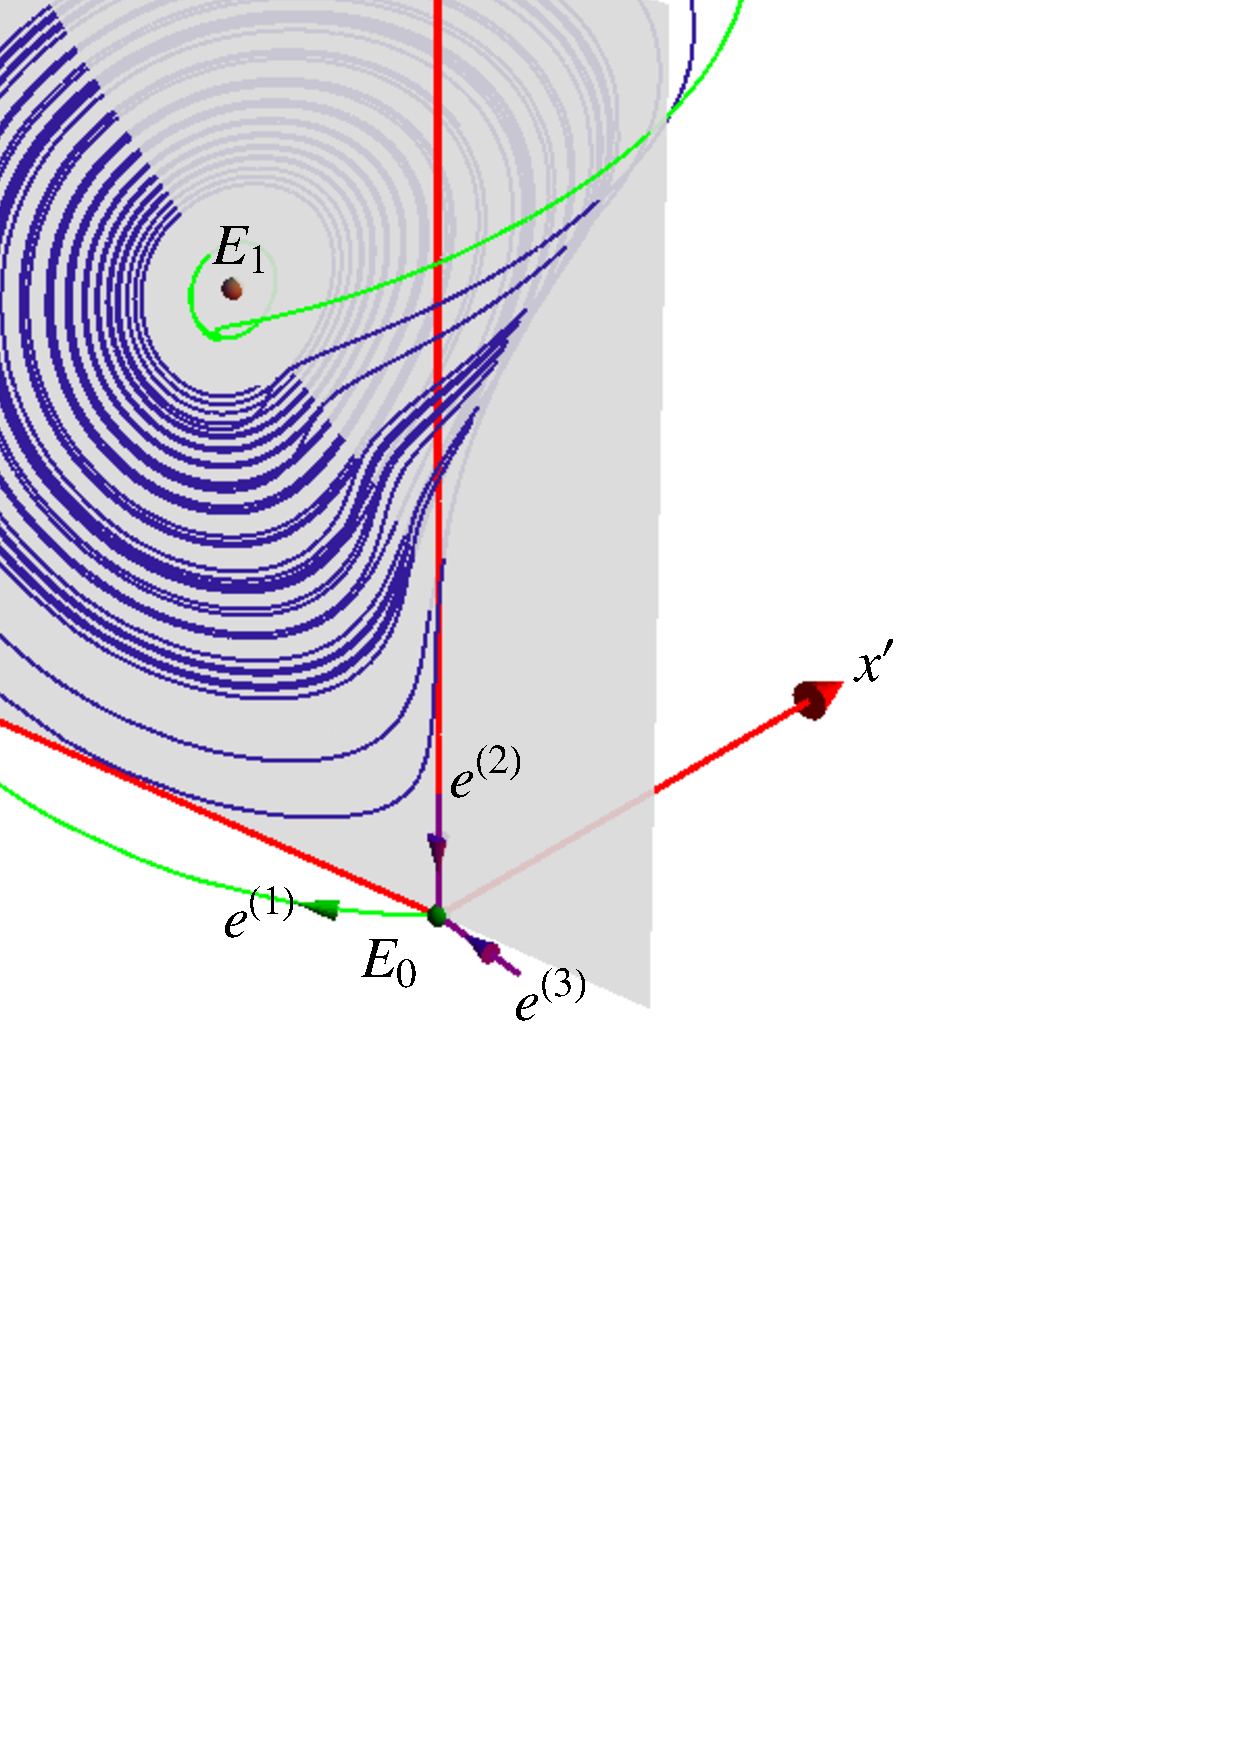
\includegraphics[width=0.40\textwidth]{../figs/lorenzPolar1}%.png}
~(b)~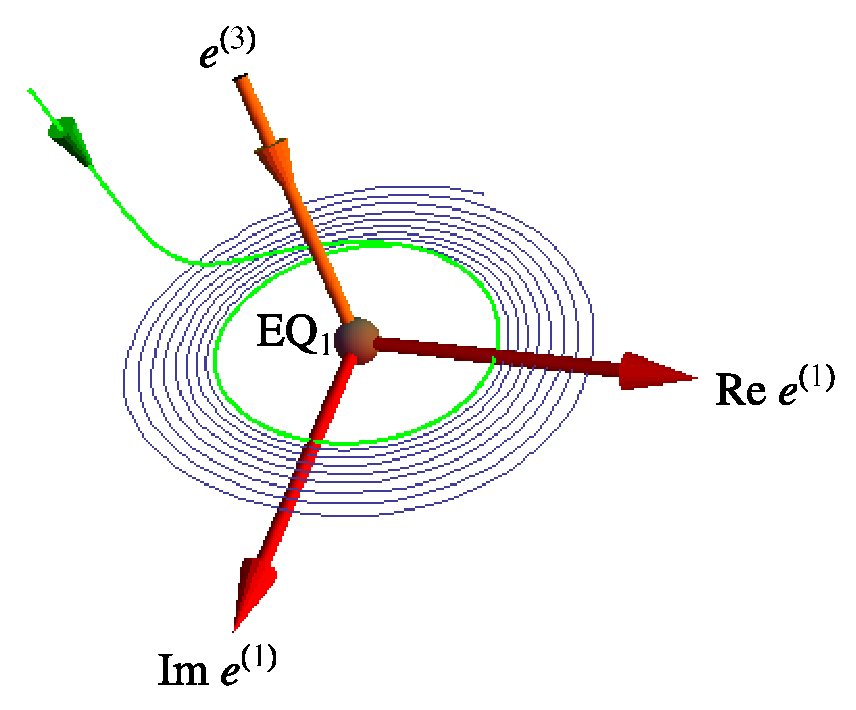
\includegraphics[width=0.44\textwidth]{../figs/lorenzPolarManifDetail1}
}{}{
(a) % $\Ztwo$-quotiented
Lorenz attractor plotted
in $[x',y',z]$, the doubled-polar angle coordinates \refeq{doubledPolar},
with points related by $\pi$-rotation in the
$[x,y]$ plane identified. Stable eigen\-vectors of $\EQV{0}$:
$\jEigvec[3]$ and $\jEigvec[2]$,
along the $z$ axis \refeq{LorenzZaxis}.
Unstable manifold orbit $W^u(\EQV{0})$
(green) is a continuation of
the unstable $\jEigvec[1]$ of $\EQV{0}$.
(b) Blow-up of the region near $\EQV{1}$:
The unstable eigenplane of $\EQV{1}$ is
defined by $\Re\jEigvec[2]$ and $\Im\jEigvec[2]$, % is shown in red, while
the stable eigen\-vector  $\jEigvec[3]$. % is shown in orange.
The descent of the
$\EQV{0}$ unstable manifold
(green) defines the innermost edge of the strange attractor.
As it is clear from (a), it also defines its outermost edge.
%(E. Siminos)
}{fig:PolarLorenz}
%%%%%%%%%%%%%%%%%%%%%%%%%%%%%%%%%%%%%%%%%%%%%%%%%%%%%%%%%%%%%%%%%%


As any such $\Rot{1/2}$-invariant section does the job, a
choice of a `fundamental domain' is here largely mater of
taste. For purposes of visualization it is convenient to make
the double-cover nature of the full \statesp\ by $\tilde{\pS}$
explicit, through any \statesp\ redefinition that maps a pair
of points related by symmetry into a single point. In case at
hand, this can be easily accomplished by expressing $(x,y)$ in
polar coordinates $(x,y) \,=\, (r \cos \theta , r \sin
\theta)$, and then plotting the flow in the
\emph{`doubled-polar angle representation:'}
\beq
(x',y') \,=\, (r \cos 2\theta , r \sin 2\theta)
        \,=\, ( (x^2-y^2)/r, 2xy/r )
\,,
\label{doubledPolar}
\eeq
as in \reffig{fig:PolarLorenz}\,(a). In contrast to the
original $G$-equivariant coordinates $[x,y,z]$, the Lorenz flow
expressed in the new coordinates $[x',y',z]$ is {\em
$G$-invariant}, see \refsect{sec:SymRPO}. In this
representation the $\tilde{\pS}=\pS/\Ztwo$ fundamental domain
flow is a smooth, continuous flow, with  (any choice of) the
fundamental domain stretched out to seamlessly  cover the
entire $[x',y']$ plane.

We emphasize: such nonlinear coordinate transformations are
\emph{not} required to implement the symmetry quotienting
$\pS/G$, unless there are computational gains in a nonlinear
coordinate change suggested by the symmetry. We offer them here
only as a visualization aid that might help the reader
disentangle 2\dmn\ projections of higher-dimensional flows. All
numerical calculations are usually carried in the initial, full
\statesp\ formulation of a flow, with symmetry-related points
identified by \emph{linear} symmetry transformations.
%~~(continued in \refsect{exmp:LorenzRetM})


\section{\Rpo s of Lorenz flow}\label{exmp:LorenzRpos}
% Predrag                           09feb2009
\index{Lorenz flow}
%(continuation of  \refsect{exmp:LorenzD1})
%
The relation between the full \statesp\ periodic orbits,
and the fundamental domain \refeq{doubledPolar} reduced orbits
of the Lorenz flow:
Full \statesp\ cycle pairs $p$, $Rp$ map into
a single cycles $\tilde{p}$ in the fundamental domain, and any
self-dual cycle $p = Rp = \tilde{p}R\tilde{p}$
is a repeat of a \rpo\ $\tilde{p}$.
%     } %end Desymmetrization of Lorenz exmp:LorenzD1
%%%%%%%%%%%%%%%%%%%%%%%%%%%%%%%%%%%%%%%%%%%%%%%%%%%%%%%%%%%%%%%%%%%%%%%%%%


%from ChaosBook.org \Chapter{knead}{19feb2009}{Charting the state space}

In this chapter we use Lorenz flows to motivate modeling of
higher-dimensional flows by iteration of 1-dimensional maps.
For these two flows the 1-dimensional maps capture essentially
all of the higher-dimensional flow dynamics, both qualitatively
and quantitatively. 1-dimensional maps suffice to explain the
two key aspects of qualitative dynamics; \emph{temporal
ordering}, or \emph{itinerary} with which a trajectory visits
\statesp\ regions, and the \emph{spatial ordering} between
trajectory points, which is the key to determining the
admissibility of an orbit with a prescribed itinerary. In a
generic dynamical system not every symbol sequence is realized
as a dynamical trajectory; as one looks further and further,
one discovers more and more rules which prohibit families of
itineraries. For 1-dimensional \stretchf\ maps the
\emph{kneading theory} provides the definitive answer as to
which temporal itineraries are {\em \admissible} as
trajectories of the dynamical system.



\subsection{From $d$-dimensional flows to
           1-dimensional maps}\label{sec:retMaps}

Symbolic dynamics for the $3$-disk game of pinball is so
straight\-forward that one may altogether fail to see the
connection between the topology of hyperbolic flows and their
symbolic dynamics. This is brought out more
clearly by the 1-dimensional visualization of \stretchf\ flows
to which we turn now.

So a typical dynamical system
that we care about is {\em bounded}. If the price to keep going
is high - for example, we try to stir up some tar, and observe
it come to a dead stop the moment we cease our labors - the
dynamics tends to settle into a simple state. However,
as the resistance to change decreases - the tar is heated up
and we are more vigorous in our stirring - the dynamics becomes
unstable.



The R\"ossler-type flows wind around the stable manifold of the
`central' \eqv, stretches and folds, and  the
flow can be reduced to a 1-dimensional map. The Lorenz flow is
similar, but the folding mechanism is very different: the unstable
manifold of one of the \eqva\ collides with the stable manifold
of the other one, forcing a robust {\em heteroclinic
connection} between the two.
    \index{heteroclinic connection}

%
%%%%%%%%%%%%%%%%%%%%%%%%%%%%%%%%%%%%%%%%%%%%%%%%%%%%%
%\PC{figs/lorenzPolarPoinc2.eps was 0.7MB - ES reduced to 14KB.
%    figs/lorenzPolarPoinc1.eps 0.8MB - now not used
\FIG{
(a)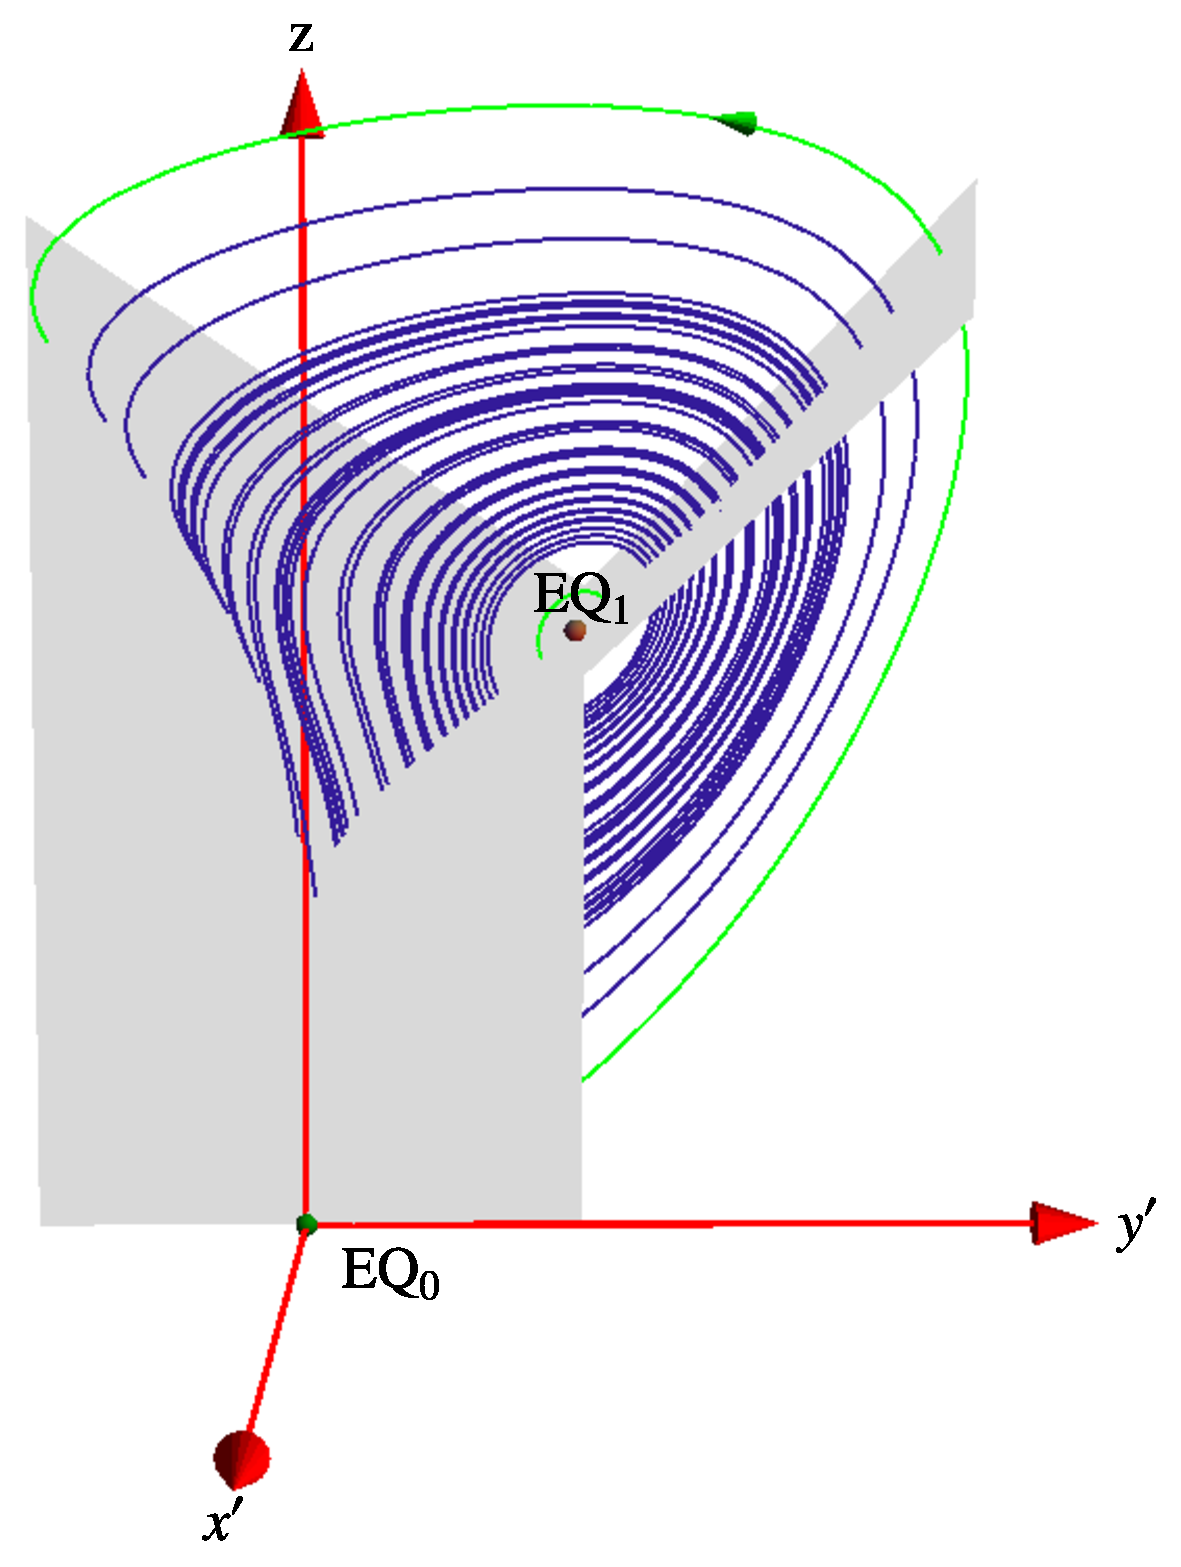
\includegraphics[width=0.42\textwidth]{../Fig/lorenzPolarPoinc2}%
~~%
(b)\raisebox{2.4ex}{
    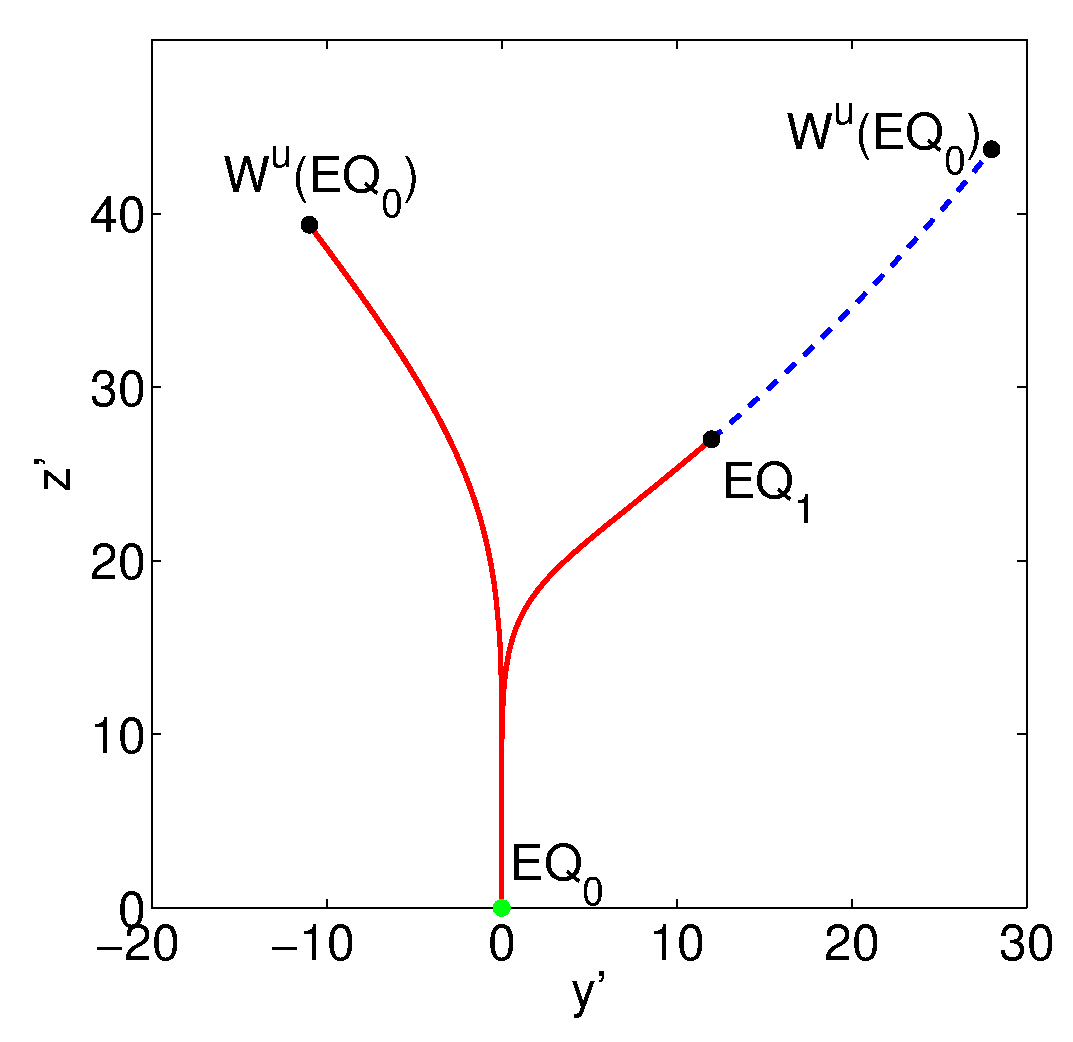
\includegraphics[width=0.44\textwidth]{../Fig/plorenz_psec}
                   }
}{}{
(a) A Poincar\'e section % $\PoincS_1$
of the Lorenz flow
in the doubled-polar angle representation, \reffig{fig:PoincLorenz},
given by the $[y',z]$ plane that contains the $z$-axis and
the \eqv\ $\EQV{1}$.
% Most of the section plane except for the
% two shaded trapezoids is removed to aid visualization of the flow.
$x'$ axis points toward the viewer.
%, with the portion of the flow piercing into
% the  section % $\PoincS_1$ shown.
%(b) The same section rotated by $\pi$ in the $[x',y']$ plane, viewed
%from above. Now the flow exiting the section % $\PoincS_1$
%is shown. This view illustrates
%the sharp folding of the outer branch, with the outermost edge
%given by the unstable manifold of $\EQV{0}$.
(b) The Poincar\'e section of the Lorenz flow by the section %$\PoincS_1$
plane (a); compare with \reffig{fig:LorenzSect}.
Crossings \emph{into} the section
are marked red (solid) and
crossings \emph{out of} the section are marked blue (dashed).
% (green dot) $\EQV{1}$ \eqv.
% (black dot) $\EQV{0}$ at the origin.
Outermost points of both in- and out-sections
are given by the $\EQV{0}$ unstable manifold $W^u(\EQV{0})$
intersections.
%(E. Siminos)
}{fig:PoincLorenz}
%%%%%%%%%%%%%%%%%%%%%%%%%%%%%%%%%%%%%%%%%%%%%%%%%%%%%%%%%%%%%%%%%%

%%%%%%%%%%%%%%%%%%%%%%%%%%%%%%%%%%%%%%%%%%%%%%%%%%%%%%%%%%%%%%%%%%
\section{Lorenz flow: Stretch \&\ crease\label{exmp:LorenzRetM}}
% Predrag                           04apr2008
% Predrag                           19jan2008
% moved to here from halcrow/blog/TEX/lorenz.tex
\index{Lorenz flow}
%
%%%%%%%%%%%%%%%%%%%%%%%%%%%%%%%%%%%%%%%%%%%%%%%%%%%%%%%%%%%%%%%%%%
% old {fig:PoincLorenz}\,(d)
\SFIG{plorenz_retmap2}
{}{
The Poincar\'e return map $s_{n+1}=\PoincM(s_n)$ parameterized by
Euclidean arclength $s$ measured along the
$\EQV{1}$ unstable manifold,
from $\ssp_{\EQV{1}}$ to  $W^u(\EQV{0})$ section point,
uppermost right point of the blue segment in
\reffig{fig:PoincLorenz}\,(b).
% PC deal with this:
% \JFGedit{(JFG: ``upper half''? I don't get it, e.g. I don't see
% how (d) is connected to what part of (c))}
The critical point (the `crease') of the map is given by
the section of the heteroclinic orbit $W^s(\EQV{0})$
that descends all the way to
$\EQV{0}$, in infinite time and with infinite slope.
}{fig:RetMapLorenz}
%%%%%%%%%%%%%%%%%%%%%%%%%%%%%%%%%%%%%%%%%%%%%%%%%%%%%%%%%%%%%%%%%%
%
We now deploy the symmetry of Lorenz flow
to streamline and complete analysis of the Lorenz strange attractor
commenced in  \refsect{exmp:LorenzD1}. There we showed that
the dihedral $D_1 = \{e,R\}$ symmetry identifies the
two \eqva\ $\EQV{1}$ and $\EQV{2}$,
and the traditional `two-eared' Lorenz flow
\reffig{LorenzAttrct} is replaced by
the `single-eared' flow
of \reffig{fig:PolarLorenz}\,(a).
Furthermore, symmetry identifies two sides of any plane
through the $z$ axis, replacing a full-space Poincar\'e
section plane by a half-plane, and the two directions
of a full-space eigen\-vector of $\EQV{0}$
 by a one-sided eigen\-vector, see \reffig{fig:PolarLorenz}\,(a).

\refExam{exmp:LorenzGlob} explained the genesis of the
$\ssp_{\EQV{1}}$ {\eqv} unstable manifold, its orientation and
thickness, its collision with the $z$-axis, and its
heteroclinic connection to the $\ssp_{\EQV{0}} = (0,\, 0,\, 0)$
{\eqv}. All that remains is to describe how the $\EQV{0}$
neighborhood connects back to the $\EQV{1}$ unstable
manifold. \refFig{fig:PolarLorenz} now shows clearly how the
Lorenz dynamics is pieced together from the 2 \eqva\ and their
unstable manifolds:

Having completed the descent to  $\EQV{0}$, the
infinitesimal neighborhood of the heteroclinic $\EQV{1} \to
\EQV{0}$ trajectory is ejected along the unstable manifold
of $\EQV{0}$ and is re-injected into the unstable manifold
of $\EQV{1}$. Both sides of the narrow strip enclosing the
$\EQV{0}$ unstable manifold  lie above it, and they get
folded onto each other with a knife-edge crease (contracted
exponentially for infinite time to the  $\EQV{0}$
heteroclinic point), with the heteroclinic out-trajectory
defining the outer edge of the strange attractor. This leads to
the folding of the outer branch of the Lorenz strange
attractor, illustrated in \reffig{fig:PoincLorenz}\,(b), with
the outermost edge following the unstable manifold of
$\EQV{0}$.

Now the stage is set for construction of  Poincar\'e sections
and associated  Poincar\'e return maps. There are two natural
choices; the section at $\EQV{0}$, lower part of
\reffig{fig:PoincLorenz}\,(b), and the section (blue) above
$\EQV{1}$. The first section, together with the blowup of
the $\EQV{0}$ neighborhood, \reffig{fig:LorenzEQ1}\,(b),
illustrates clearly the scarcity of trajectories (vanishing
natural measure) in the neighborhood of $\EQV{0}$. The flat
section above $\EQV{1}$ (which is, believe it or not, a
smooth conjugacy by the flow of the knife-sharp section at
$\EQV{0}$) is more convenient for our purposes. Its return
map is given by \reffig{fig:RetMapLorenz}.

The rest is straight sailing: to accuracy $10^{-4}$ the return
map is unimodal, its critical point's forward trajectory
yields the \ks, and the \admissible\ binary
sequences, so any number of periodic points  can be accurately
determined from this 1-dimensional return map, and the 3\dmn\
cycles then verified by integrating the Lorenz differential
equations \refeq{Lorenz}. The map is everywhere expanding on
the strange attractor, so it is no wonder mathematicians can
here make the ergodicity rigorous.
    %
    \PC{Paragraph here - codimensionality of manifolds from
        paper with Viswanath}

What have we learned from the above two exemplary 3-dimensional
flows? If a flow is locally unstable but globally bounded, any
open ball of initial points will be stretched out and then
folded back. If the \eqva\ are hyperbolic, the trajectories
will be attracted along some eigen-directions and ejected along
others. The unstable manifold of one \eqv\ can avoid stable
manifolds of other \eqva, as is the case for R\"ossler, or
slice them head on, as is the case for Lorenz. Hence
qualitatively a typical trajectory will wander through
\statesp, being alternatively attracted into \eqva\
neighborhoods, and then ejected again. What is important is the
motion along the unstable manifolds --that is where
1-dimensional maps come from.
